% Neurocomputing submission entry point.
\documentclass[preprint,12pt]{elsarticle}

\usepackage{amsmath,amssymb,amsfonts,amsthm}
\usepackage{array}
\usepackage{booktabs}
\usepackage{graphicx}
\usepackage{multirow}
\usepackage{textcomp}
\usepackage{xcolor}
\usepackage{url}
\usepackage[hidelinks]{hyperref}

\graphicspath{{code/figures/}{figures/}}

\newtheorem{theorem}{Theorem}
\newtheorem{proposition}{Proposition}
\newtheorem{definition}{Definition}
\newtheorem{remark}{Remark}
\newtheorem{corollary}{Corollary}
\newtheorem{lemma}{Lemma}
\newtheorem{assumption}{Assumption}

\journal{Neurocomputing}

\begin{document}

\begin{frontmatter}

\title{A Prospective Evaluation of Simple Graph Diagnostics for Graph-vs-MLP Model Selection}

\author{Anonymous Author(s)}
\affiliation{organization={Anonymous institution},
             city={Anonymous},
             country={Anonymous}}

\begin{abstract}
Choosing whether to use graph structure is an operational decision, yet graph statistics are usually evaluated as correlates of performance rather than as decision rules. We test whether transparent diagnostics whose label-dependent graph statistics use training labels only can select between tuned graph and feature-only multilayer perceptron (MLP) portfolios for node classification. Before generating these confirmatory records, we freeze datasets, splits, seeds, seven architectures, four-trial grids, the practical margin, label scope, abstention, and analysis. The comparison uses asymmetric portfolios: six graph architectures receive 24 trials, whereas one MLP architecture receives four. An outcome-independent eligibility amendment excludes one dataset whose singleton class cannot support the frozen three-way split; all scientific settings remain unchanged. The final benchmark contains 11 datasets, 110 dataset--seed units, 770 model records, and 110 diagnostic records without failed units. The combined diagnostic attains 55.5\% selection accuracy, 68.2\% coverage, and 7.46 percentage points of full-set regret. Always-graph attains 80.9\% accuracy and 0.26 points of regret; validation selection attains 91.8\% and 0.22 points. Dataset-level paired comparisons do not establish an advantage for the combined diagnostic after Holm correction. A separate degree-preserving randomization on Cora, CiteSeer, and PubMed reduces GCN accuracy by 45.5, 29.9, and 17.3 points, respectively. Diagnostic failure therefore should not be read as evidence that edge organization is uninformative, although the intervention does not isolate homophily or another single mechanism. Under this protocol, simple diagnostics do not reliably choose between the evaluated graph and MLP portfolios.
\end{abstract}

\begin{keyword}
graph neural networks \sep model selection \sep graph diagnostics \sep heterophily \sep negative results
\end{keyword}

\end{frontmatter}

% ============================================================
% Section 1: Introduction
% Negative diagnostic study: frozen graph-vs-MLP family selection
% ============================================================

\section{Introduction}
\label{sec:intro}

Graph Neural Networks (GNNs) can exploit relational information that a feature-only model cannot access, but using the graph is not uniformly beneficial~\cite{kipf2017gcn,velivckovic2018gat,hamilton2017graphsage}. This creates a practical decision before deployment: should a node-classification task use a graph-model portfolio or a feature-only multilayer perceptron (MLP) portfolio? Training and validating both portfolios can answer the question retrospectively, but a cheap diagnostic would be valuable when training and tuning the graph-model portfolio is costly. The graph is already available in this setting because both the candidate models and the structural diagnostics use it.

Existing work shows why this decision is difficult. Homophily alone does not characterize GNN performance, and recent metrics incorporate class-conditional, feature, structural, or neighborhood-distribution information~\cite{luan2023whendo,platonov2023characterizing,zheng2024trihom,pmlr-v235-wang24u}. Other work treats graph-model selection as a cross-dataset meta-learning problem~\cite{park2023metagl,park2023glemos}. These studies establish that graph characteristics can correlate with performance and that learned selectors can rank graph models. They do not, however, determine whether a fixed set of transparent statistics, with label-dependent graph quantities restricted to the training split, is reliable enough to support an explicit graph-versus-MLP family action under matched trivial and validation-based policies.

Correlation is not the same as a safe decision. A statistic can correlate with a performance gap yet still produce costly errors at a fixed threshold; a high selection accuracy can also be misleading when one action dominates the benchmark. We therefore evaluate diagnostics as policies with three outputs---graph, MLP, or abstain---and measure oracle-portfolio regret, coverage, and selection accuracy. The target selects graph only when the tuned graph portfolio exceeds the tuned MLP by more than a predeclared one-percentage-point margin; all smaller gaps map to MLP. Regret remains primary because graph is the target on 89 of the 110 evaluation units.

We conduct a frozen prospective evaluation on newly generated confirmatory records rather than redesign the rule after observing their comparative outcomes. Before generating those records, we fix the candidate datasets, ten seeds, 60/20/20 splits, seven architectures, four tuning trials per architecture, diagnostic label scope, thresholds, tie handling, MLP fallback for abstention, and dataset-level inference. Historical aggregate results had been inspected during earlier exploratory work, but they are excluded from the confirmatory benchmark. A feasibility-aborted v1 run reveals that Texas has a singleton class and cannot support the frozen per-class three-way split. Before any comparative benchmark was assembled or evaluated, an outcome-independent eligibility amendment excludes Texas, assigns a new run identifier, and restarts all remaining datasets from zero without changing the scientific settings. The final 11-dataset artifact contains 770 model records and 110 train-only diagnostic records with no failed evaluation units. The combined diagnostic is compared on identical units with always-graph, always-MLP, random 50/50, homophily-only, degree-only, homophily-plus-degree, two-hop-only, and direct validation-selection policies.

The prospective result is negative and operationally consequential. The combined diagnostic reaches 55.5\% selection accuracy at 68.2\% coverage and incurs 7.46 percentage points of full-set regret. Always-graph reaches 80.9\% accuracy with 0.26 points of regret, while validation selection reaches 91.8\% accuracy with 0.22 points of regret. None of the eight predeclared comparisons establishes an advantage for the combined rule after Holm correction. The evaluated diagnostics therefore provide no stable incremental value for graph-vs-MLP selection under this protocol.

This failure does not imply that graph structure is irrelevant. In a separate frozen intervention, degree-preserving randomization reduces GCN test accuracy by an average of 45.5 points on Cora, 29.9 on CiteSeer, and 17.3 on PubMed. The intervention preserves every node's degree but jointly changes class mixing, connectivity patterns, and higher-order organization; it therefore supports an edge-organization interpretation without isolating homophily as a causal mechanism. The two experiments together expose the central gap: useful graph signal can be substantial even when simple statistics fail to characterize when a graph model should be used.

The paper makes three contributions:
\begin{enumerate}
    \item \textbf{A frozen graph-vs-MLP decision benchmark.} We evaluate transparent diagnostics---with label-dependent graph statistics restricted to the training split and no test-label access---as explicit actions under fixed asymmetric model portfolios, matched per-architecture tuning grids, common splits and seeds, a practical margin, and test-once accounting.
    \item \textbf{A decision-oriented negative result.} Across 110 units, simple diagnostics do not improve on trivial policies in a stable way; regret and coverage reveal failures that correlation or raw accuracy alone can obscure.
    \item \textbf{A mechanism--decision separation.} A degree-preserving paired intervention shows that diagnostic failure cannot be reduced to graph irrelevance, while a scoped discriminability calculation in Section~\ref{sec:snr} provides limited mechanistic context without serving as a selection theorem.
\end{enumerate}

The remainder of the paper positions the study against graph characterization and model selection, defines the frozen decision protocol, reports the prospective benchmark and intervention, and then presents scoped mechanistic context and limitations.

% ============================================================
% Section 2: Related Work
% Negative diagnostic study: closest-work positioning
% ============================================================

\section{Related Work}
\label{sec:related}

The study sits at the intersection of graph-characterization metrics, heterophilous node classification, graph learning model selection, and tests of whether graph structure is necessary. Its contribution is a frozen decision evaluation of simple diagnostics, not a new homophily measure, graph architecture, or general model-selection benchmark.

\subsection{Graph Characteristics and Relative Model Performance}

Early homophily measures summarize whether adjacent nodes share labels, but a single global fraction omits class imbalance, feature geometry, neighborhood distributions, and local variation~\cite{mcpherson2001homophily,zhu2020beyond,ma2021homophily}. Subsequent work introduced post-aggregation similarity, adjusted homophily, label informativeness, and local or class-conditional characterizations to better describe when message passing helps~\cite{luan2022linkx,platonov2023characterizing,loveland2024local}. Accordingly, our contribution is not the established observation that homophily is insufficient.

The closest diagnostic work goes further. Luan et al.~\cite{luan2023whendo} analyze node distinguishability and propose feature-based hypothesis-testing metrics with thresholds intended to reveal the advantage of graph-aware models. Zheng et al.~\cite{zheng2024trihom} disentangle label, structural, and feature homophily; their 31-dataset study compares Tri-Hom with 17 metrics, including correlations with GCN-, GraphSAGE-, and GAT-versus-MLP performance gaps. Under a heterophilous stochastic block model, Wang et al.~\cite{pmlr-v235-wang24u} relate separability gain to neighborhood-distribution distance and degree rather than to global homophily alone. These studies motivate richer diagnostics but primarily evaluate theoretical quantities or performance association. We instead freeze specified statistics as graph/MLP/abstain policies and evaluate the cost of their actions through regret and coverage.

Benchmark design also narrows the novelty claim. Repeated-split evaluation and standardized graph collections expose conclusions that depend on data splits, tuning, or dataset choice~\cite{shchur2018pitfalls,hu2020ogb}. Platonov et al.~\cite{platonov2023heterophilous} reassess whether reported progress on heterophilous benchmarks survives stronger protocols, while Luan et al.~\cite{luan2024reevaluating} quantitatively re-evaluate both models and homophily metrics. Comparisons across datasets further require treating datasets, rather than pooled seeds, as the inferential units~\cite{demsar2006statistical}. We therefore do not claim the first negative evaluation of homophily-related diagnostics. Our narrower question is whether transparent train-only rules retain incremental decision value over matched trivial policies on real dataset--seed units when negative outcomes are preserved without threshold redesign.

\subsection{Heterophily-Aware Architectures}

Heterophily-aware models change which signals are propagated or how they are combined. H2GCN separates ego and neighbor representations and uses two-hop neighborhoods~\cite{zhu2020beyond}; LINKX separates structural and feature processing~\cite{luan2022linkx}; MixHop and GPR-GNN combine multiple propagation depths~\cite{abu2019mixhop,chien2021gprgnn}; FAGCN, GloGNN, and ACM-GCN adapt filters or communication patterns~\cite{fagcn2021,li2022glognn,acmgcn2024}. Geom-GCN constructs geometric neighborhoods, while high-frequency and flexible spectral designs broaden the signals a graph model can retain~\cite{pei2020geomgcn,he2022bernnet,wang2022jacobi}. The wider node-classification design space also includes simplified propagation, deeper residual propagation, revised attention, and graph-augmented MLPs~\cite{wu2019sgc,chen2020gcnii,brody2022gatv2,zhang2021gamlp}. These architectures demonstrate that low one-hop homophily need not make graph structure useless. They also make architecture-specific prediction difficult: a statistic that describes one-hop mixing need not identify which portfolio wins after tuning. Our benchmark therefore places GCN, GAT, GraphSAGE, H2GCN, LINKX, and GPR-GNN in the graph portfolio and evaluates a portfolio action rather than presenting a new heterophily architecture.

Depth introduces a separate limitation: repeated propagation can erase discriminative variation or contract node representations~\cite{oono2020exponential,chen2020measuring}. DropEdge and PairNorm address this behavior through edge sampling and representation normalization~\cite{rong2020dropedge,zhao2020pairnorm}. These results reinforce the distinction between describing a graph and forecasting the outcome of a tuned portfolio: realized graph utility depends jointly on data, architecture, optimization, and regularization.

\subsection{Graph Learning Model Selection}

Graph model selection has been studied directly. Auto-GNN searches neural architectures for a given graph task~\cite{zhou2020autognn}. MetaGL learns to select graph-learning models on a new graph from meta-graph features and historical performance~\cite{park2023metagl}. GLEMOS scales this problem to 366 models and 457 graphs and benchmarks multiple instantaneous selection algorithms~\cite{park2023glemos}. Consequently, the present 11-dataset experiment is neither the first nor the largest graph-model-selection benchmark.

Our estimand differs from ranking many individual models across a large meta-dataset. We ask whether predeclared, interpretable statistics can support a binary graph-portfolio-versus-MLP-portfolio action without using test labels. Each architecture receives the same four-trial validation grid, but the total search budgets are not equal: the graph action selects among six architectures and the feature-only action contains one MLP. The final test outcome is evaluated once, and the diagnostic rules are compared with always-graph, always-MLP, random, and direct validation-selection policies on the same 110 units. This design treats diagnostics as deployable decisions and makes oracle-portfolio regret and abstention coverage explicit.

\subsection{When Is the Graph Necessary?}

Strong feature-only baselines are essential because some graph benchmarks can be solved largely from node features. Prior studies have documented competitive MLPs, evaluation instability, and feature leakage of graph information~\cite{huang2021mlp,shchur2018pitfalls,katsman2026necessary}. Other controls compare predictions with and without meaningful edges, showing that models can exploit graph structure when it hurts generalization~\cite{bechler2024graphs}. These findings motivate the graph-versus-MLP action but do not supply a cheap rule for making it.

Our intervention complements these controls. It holds every node's degree fixed while randomizing edge organization. It does not isolate homophily: class mixing, paths, components, clustering, and other higher-order properties can change together. We use the intervention only to reject the interpretation that diagnostic failure demonstrates graph irrelevance. The main contribution remains the decision audit: graph signal may matter strongly even when the evaluated statistics cannot identify its utility reliably.

\subsection{Scoped Mechanistic Context}

The fixed-degree Gaussian calculation in Section~\ref{sec:snr} is included to explain why correlation, degree, and feature strength can interact under a prescribed linear average. It is adjacent to contextual stochastic-block-model recovery theory and finite-depth embedding analyses~\cite{lu2023contextual,pmlr-v269-dalle25a}, but it is not a new recovery threshold, Bayes-error result, or trained-GNN guarantee. The negative benchmark does not depend on that calculation being a universal theory; it evaluates the diagnostics directly under the frozen empirical protocol.

\section{Decision Problem and Frozen Protocol}
\label{sec:protocol}

\subsection{Graph-vs-MLP Decision}

The unit of evaluation is a dataset--seed pair $u$. Within each unit, validation performance selects one feature-only MLP and one graph model from GCN, GAT, GraphSAGE, H2GCN, LINKX, and GPR-GNN. Every architecture receives the same four-trial tuning budget, and exact validation ties are broken by model identifier. Let $a_u^{\mathrm{M}}$ and $a_u^{\mathrm{G}}$ denote the held-out test accuracies of the selected MLP and graph model. The evaluator reads each selected test result once; no diagnostic can affect training or hyperparameter selection.

We ask whether the graph family provides a practically material gain rather than whether it wins by an arbitrarily small amount. With the frozen margin $\delta=0.01$, the target action is
\begin{equation}
y_u =
\begin{cases}
\mathrm{G}, & a_u^{\mathrm{G}}-a_u^{\mathrm{M}}>\delta,\\
\mathrm{M}, & a_u^{\mathrm{G}}-a_u^{\mathrm{M}}\leq\delta.
\end{cases}
\label{eq:decision_target}
\end{equation}
The same tie policy applies to every evaluated rule. This formulation makes the decision asymmetric by design: a graph model must exceed the MLP by more than one percentage point to justify the graph action.

\subsection{Matched Training and Selection}

Table~\ref{tab:frozen_training} records the common training budget from the frozen machine-readable specification. The implementation uses PyTorch~\cite{paszke2019pytorch}, and each trial minimizes cross-entropy with Adam. Early stopping retains the checkpoint with the highest validation accuracy, then the lowest validation loss and earliest epoch; training stops after 100 stale epochs or 500 epochs in total. The four trial configurations are selected independently within every architecture, and the chosen checkpoint then receives one held-out test evaluation. Thus no model family obtains a larger search budget or repeated access to the test split.

\begin{table}[t]
\centering
\caption{Frozen Matched Training Configuration}
\label{tab:frozen_training}
\small
\begin{tabular}{@{}lp{0.64\linewidth}@{}}
\toprule
Component & Frozen setting \\
\midrule
Representation width & 64 hidden channels for every architecture. \\
Optimization & Adam, cross-entropy loss, weight decay $5\times 10^{-4}$. \\
Training horizon & At most 500 epochs; patience 100 under the validation checkpoint rule. \\
Four-trial grid & Learning rate in $\{0.01,0.005\}$ crossed with dropout in $\{0.5,0.7\}$. \\
Model-specific constants & GAT: 4 heads; H2GCN: 2 propagation layers with strict two-hop edges; LINKX: 2 outer, 1 edge, and 2 node layers; GPR-GNN: 10 propagation steps, $\alpha=0.1$, PPR initialization. \\
Selection and test & Validation accuracy descending, validation loss ascending, trial identifier ascending; one held-out test evaluation. \\
\bottomrule
\end{tabular}
\end{table}

The split is stratified 60/20/20 for train/validation/test and is regenerated deterministically for seeds 0--9. Every unit stores the source commit, canonical configuration digest, processed-data checksums, split identifier, four trial records, selected checkpoint, and environment provenance. The v1 and v2 JSON specifications differ only in the pre-outcome eligibility amendment described in Section~\ref{sec:prospective}; the later Squirrel amendment changes only the execution timeout.

AI-assisted tools supported software review, test development, reproducibility checks, and editorial work but did not generate experimental data or make reporting decisions. All reported experiments were executed under the frozen protocol, and the author independently verified the code, artifacts, analyses, and manuscript claims.

\subsection{Decision-Time Information and Policies}

Full node features and graph structure are available because they are model inputs. Label-dependent graph statistics may use training labels only. In particular, edge homophily uses edges whose endpoints are both labeled for training, and the two-hop statistic uses training-labeled endpoint pairs. Validation accuracy is available because model tuning precedes the decision. Test labels, test accuracy, and any statistic computed from test labels are forbidden diagnostic inputs; the evaluator rejects records that violate this boundary.

Table~\ref{tab:diagnostic_policies} lists the nine frozen policies. The thresholds are historical or deliberately simple sanity baselines; none is fitted to the prospective outcomes. The combined policy chooses graph when training-only edge homophily is at least $0.55$. Below that threshold, it chooses MLP when MLP validation accuracy is at least $0.40$ and otherwise abstains. Missing diagnostic inputs also cause abstention. For full-set evaluation, every abstention uses the same predeclared MLP fallback, while coverage remains separately visible.

\begin{table}[t]
\centering
\caption{Frozen Graph-vs-MLP Decision Policies}
\label{tab:diagnostic_policies}
\small
\begin{tabular}{@{}lp{0.67\linewidth}@{}}
\toprule
Policy & Decision rule \\
\midrule
Always-MLP & Select MLP for every unit. \\
Always-graph & Select the validation-chosen graph model for every unit. \\
Random 50/50 & Use the analytic expectation of equally likely graph and MLP actions. \\
Homophily-only & Select graph when training-only edge homophily is at least $0.50$. \\
Degree-only & Select graph when mean degree is at least $10$. \\
Homophily+degree & Threshold the equal-weight sum of centered homophily and log-degree scores at zero. \\
Two-hop-only & Select graph when training-only $h_2-h_1>0.05$. \\
Combined & Apply the historical homophily/MLP-validation rule described in the text; otherwise abstain. \\
Validation selection & Select graph when its validation advantage exceeds $\delta$. \\
\bottomrule
\end{tabular}
\end{table}

\subsection{Outcomes and Inference}

Selection accuracy measures agreement with Eq.~\eqref{eq:decision_target} after the common fallback, and coverage is the fraction of non-abstaining decisions. Because an incorrect action can have negligible or substantial cost, the primary loss is oracle-family regret,
\begin{equation}
r_u(\widehat{y})=\max\{a_u^{\mathrm{G}},a_u^{\mathrm{M}}\}-a_u^{\widehat{y}},
\label{eq:oracle_regret}
\end{equation}
where $a_u^{\widehat{y}}$ is the test accuracy of the chosen family after fallback. We report mean full-set regret for all units and covered-set regret for non-abstaining units. Risk--coverage curves order decisions by each policy's frozen confidence score.

Seeds remain paired within a dataset. We first average regret over seeds for each dataset, then use the dataset means for percentile-bootstrap intervals and two-sided sign-flip tests. Holm correction controls the family-wise error rate across the eight predeclared comparisons with the combined policy. Non-significance is not interpreted as equivalence.

The prospective specification, immutable per-unit schema, analysis code, bootstrap seed, permutation seed, and paper-level decision rule were fixed before assembling or evaluating the new comparative outcomes. Section~\ref{sec:prospective} reports two outcome-independent protocol amendments and keeps the earlier feasibility artifacts outside the final analysis.

\section{Prospective Benchmark Results}
\label{sec:prospective}

\subsection{Scope and Audit Trail}

The final benchmark contains 11 datasets. Cora, CiteSeer, PubMed, and Coauthor-CS represent citation and co-authorship graphs; Chameleon, Squirrel, Actor, Wisconsin, Cornell, Roman-empire, and Amazon-ratings broaden the structural regimes. Each dataset uses ten fixed seeds, with 60\% of nodes for training, 20\% for validation, and 20\% for testing. The run yields 770 selected-model records and 110 diagnostic records: every unit contains the MLP and six graph architectures, four tuning trials per architecture, explicit split and environment provenance, and one test evaluation after validation selection. No final-run unit fails.

The execution history contains two documented amendments. First, the v1 feasibility run stops before model training on Texas because one class contains a single node and cannot populate the frozen three-way split. Before comparative assembly or evaluation, an outcome-independent eligibility amendment excludes Texas, assigns a new run identifier, and restarts all remaining datasets from zero without changing models, splits, seeds, thresholds, metrics, or inference. Second, after a blinded wall-clock timeout on Squirrel, an execution-only amendment increases the per-dataset limit from 30 to 90 minutes. No comparative outcome is inspected, and all scientific settings remain unchanged. The completed v2 artifacts retain the amendments and exclude the aborted v1 records from analysis.

\subsection{Primary Policy Outcomes}

Graph is the target action in 89 of 110 units, so a selector must be compared with the trivial always-graph policy rather than judged by raw accuracy alone. Table~\ref{tab:prospective_policy_results} reports every frozen policy on identical units. The historical combined diagnostic reaches 55.5\% selection accuracy at 68.2\% coverage. Its covered decisions incur 2.64 percentage points of regret, but the common MLP fallback on 35 abstentions raises full-set regret to 7.46 points.

\begin{table}[t]
\centering
\caption{Prospective Graph-vs-MLP Policy Results on 110 Dataset--Seed Units. Regret is reported in percentage points; selection accuracy uses the common MLP fallback.}
\label{tab:prospective_policy_results}
\small
\begin{tabular}{@{}lccc@{}}
\toprule
Policy & Accuracy (\%) & Coverage (\%) & Regret (pp) \\
\midrule
Combined & 55.5 & 68.2 & 7.46 \\
Always-graph & 80.9 & 100.0 & 0.26 \\
Always-MLP & 19.1 & 100.0 & 9.69 \\
Random 50/50 & 50.0 & 100.0 & 4.97 \\
Homophily-only & 55.5 & 100.0 & 7.46 \\
Degree-only & 37.3 & 100.0 & 6.24 \\
Homophily+degree & 46.4 & 100.0 & 5.80 \\
Two-hop-only & 28.2 & 100.0 & 8.27 \\
Validation selection & 91.8 & 100.0 & 0.22 \\
\bottomrule
\end{tabular}
\end{table}

Always-graph attains 80.9\% selection accuracy and 0.26 points of regret. Direct validation selection attains 91.8\% and 0.22 points, respectively. Homophily-only has the same full-set accuracy and regret as the combined policy after fallback, while degree-only, homophily-plus-degree, and two-hop-only also fail to improve on always-graph. The result is therefore not that a different fixed threshold rescues the original idea; under this portfolio and target, the evaluated low-dimensional rules provide no stable incremental decision value.

\subsection{Paired Inference and Interpretation}

Relative to the combined diagnostic, the dataset-level mean regret difference is $-7.20$ points for always-graph. Its 95\% bootstrap interval is $[-13.17,-1.70]$, with a raw sign-flip $p$-value of $0.015625$. The difference for validation selection is $-7.24$ points, with interval $[-13.18,-1.78]$ and raw $p=0.03125$. After Holm correction across all eight comparisons, the adjusted values are $0.125$ and $0.21875$. We therefore do not claim confirmatory superiority for either reference policy, and we do not treat the non-significant adjusted tests as equivalence.

The operational conclusion is narrower and does not depend on a significance claim in the opposite direction. The combined rule fails its predeclared incremental-value criterion because it does not reduce regret relative to simple policies and its uncertainty does not establish an advantage. Selection accuracy alone would hide this result: the target imbalance makes always-graph strong, while regret shows that the diagnostic's errors are also substantially more costly. Section~\ref{sec:edge_intervention} next tests whether this failure can be explained by graph structure being uninformative.

\section{Degree-Preserving Edge Intervention}
\label{sec:edge_intervention}

\subsection{Paired Intervention Design}

Diagnostic failure could arise either because graph structure carries little predictive information or because the evaluated statistics do not capture its useful organization. We distinguish these explanations with a separate intervention on Cora, CiteSeer, and PubMed. For each dataset and seed, verified double-edge swaps randomize the graph while preserving the complete node set, edge count, and degree of every node. The runner stores both edge lists and recomputes the simple-graph, self-loop, duplicate-edge, per-node-degree, connectivity, and homophily checks before training.

The original and randomized conditions use the same node features, labels, split, GCN architecture, and four-trial hyperparameter grid. They select hyperparameters independently by validation accuracy and evaluate the selected test state once. The paired estimand is randomized minus original test accuracy for the same dataset, split, and seed. This design isolates sensitivity to edge organization beyond the degree sequence, but it does not isolate a single changed property: swaps jointly alter class mixing, connectivity patterns, motifs, and higher-order neighborhoods.

\subsection{Results}

\begin{table}[t]
\centering
\caption{Degree-Preserving Edge-Randomization Results. Differences and confidence intervals are percentage points.}
\label{tab:degree_intervention}
\small
\begin{tabular}{@{}lcccc@{}}
\toprule
Dataset & Original (\%) & Randomized (\%) & Difference & 95\% CI \\
\midrule
Cora & 88.0 & 42.4 & $-45.5$ & $[-47.2,-44.1]$ \\
CiteSeer & 77.2 & 47.4 & $-29.9$ & $[-30.6,-29.1]$ \\
PubMed & 87.3 & 69.9 & $-17.3$ & $[-17.8,-16.9]$ \\
\bottomrule
\end{tabular}
\end{table}

All 30 paired seed differences are negative. The seed-level two-sided sign-flip tests yield Holm-adjusted $p=0.005859$ for each dataset. The equal-weight mean across the three dataset effects is $-30.9$ points, with a descriptive dataset-bootstrap interval of $[-45.5,-17.3]$. However, three dataset clusters provide only eight possible sign patterns; the exact dataset-cluster sign-flip test gives $p=0.25$.

These results rule out a simple graph-irrelevance interpretation on the three evaluated citation networks: changing edge organization while holding every node degree fixed materially changes GCN accuracy. They do not show that homophily alone causes the change, establish the same effect outside these datasets, or validate any diagnostic threshold. Together with Section~\ref{sec:prospective}, the intervention supports a mechanism--decision separation: edge organization can matter greatly even when simple graph summaries fail to indicate when a graph model should be used.

% ============================================================
% Scoped aggregation discriminability analysis
% Target: ~4 pages
% ============================================================

\section{Scoped Mechanistic Context: Aggregation Discriminability}
\label{sec:snr}

The prospective benchmark shows that the evaluated graph statistics are inadequate selection rules; it does not explain which interactions those summaries omit. As limited mechanistic context, we isolate how a linear aggregation operator changes class-conditional first and second moments in a binary fixed-degree surrogate. The calculation is exact for the stated conditional-neighbor model, but it is not an information-theoretic error bound, a model-selection rule, or a guarantee for a trained GNN.

\begin{table}[t]
\centering
\caption{Key Notation Used in This Section}
\label{tab:notation}
\small
\begin{tabular}{@{}cl@{}}
\toprule
\textbf{Symbol} & \textbf{Definition} \\
\midrule
$\rho$ & Conditional neighbor-label correlation, $\rho\in[-1,1]$ \\
$d$ & Fixed number of aggregated neighbors \\
$s$ & Feature strength, $s=\mu^\top\Sigma^{-1}\mu$ \\
$\kappa$ & Exact discriminability ratio in Proposition~\ref{prop:fixed_degree} \\
$\alpha$ & Weight on the center-node feature, $\alpha\in[0,1]$ \\
$\mathcal{D}(Z)$ & Moment-based Mahalanobis discriminability of $Z$ \\
$\Delta_Z$ & Class separation, $\mathbb{E}[Z|Y=+1] - \mathbb{E}[Z|Y=-1]$ \\
$\Sigma_Z$ & Within-class covariance, $\mathrm{Cov}(Z|Y)$ \\
\bottomrule
\end{tabular}
\end{table}

\subsection{Problem Setup}

Let the center label be $Y_v\in\{-1,+1\}$ with equal class prior and let
\begin{equation}
    X_v=Y_v\mu+\varepsilon_v,
    \qquad \varepsilon_v\sim\mathcal{N}(0,\Sigma),
\end{equation}
where $\Sigma\succ0$, $\mu\neq0$, and noises are independent across nodes. Conditional on $Y_v=y$, the $d\geq1$ neighbor labels are independent and satisfy
\begin{equation}
    \mathbb{P}(Y_i=y\mid Y_v=y)=\frac{1+\rho}{2}.
\end{equation}
Thus $\mathbb{E}[Y_i\mid Y_v=y]=\rho y$ and $\operatorname{Var}(Y_i\mid Y_v=y)=1-\rho^2$. In a balanced binary graph with a uniform conditional neighbor mechanism, $\rho$ corresponds to $2h-1$; the derivation itself is conditional and does not replace a random graph degree by its mean.

\begin{definition}[Moment-Based Discriminability]
\label{def:discriminability}
Suppose the two classes have the same nonsingular conditional covariance $\Sigma_Z$. We define the moment-based discriminability of representation $Z$ as
\begin{equation}
    \mathcal{D}(Z) := \Delta_Z^\top \Sigma_Z^{-1} \Delta_Z
\end{equation}
where $\Delta_Z = \mathbb{E}[Z|Y=+1] - \mathbb{E}[Z|Y=-1]$. This quantity uses only the first two conditional moments. It is not, in general, a distance between the full class-conditional distributions.
\end{definition}

\subsection{Exact Fixed-Degree Calculation}

We first analyze a deliberately restricted model without replacing a random degree by its expectation. Conditional on a center label $Y_v=y$, let $Y_1,\ldots,Y_d$ be independent neighbor labels satisfying $\mathbb{P}(Y_i=y\mid Y_v=y)=(1+\rho)/2$. Let $X_i=Y_i\mu+\varepsilon_i$, where the $\varepsilon_i\sim\mathcal{N}(0,\Sigma)$ are independent of all labels, and define $A_v=d^{-1}\sum_{i=1}^d X_i$.

\begin{proposition}[Exact Fixed-Degree Discriminability]
\label{prop:fixed_degree}
For $s=\mu^\top\Sigma^{-1}\mu>0$, the conditional moments and discriminability ratio are
\begin{align}
    \mathbb{E}[A_v\mid Y_v=y] &= \rho y\mu,\\
    \operatorname{Cov}(A_v\mid Y_v=y)
        &= \frac{1}{d}\left(\Sigma+(1-\rho^2)\mu\mu^\top\right),\\
    \kappa(d,\rho,s)
        :=\frac{\mathcal{D}(A)}{\mathcal{D}(X)}
        &=\frac{\rho^2d}{1+(1-\rho^2)s}.
\end{align}
\end{proposition}

\begin{proof}
We derive this result in three steps.

Since $\mathbb{E}[Y_i\mid Y_v=y]=\rho y$ and
$\operatorname{Var}(Y_i\mid Y_v=y)=1-\rho^2$, independence gives the first two identities. Moreover, $\Delta_X=2\mu$, $\mathcal{D}(X)=4s$, and $\Delta_A=2\rho\mu$. Applying the Sherman--Morrison identity,
\begin{equation}
 \mu^\top\left(\Sigma+(1-\rho^2)\mu\mu^\top\right)^{-1}\mu
 =\frac{s}{1+(1-\rho^2)s}.
\end{equation}
Substitution yields the stated ratio.
\end{proof}

\subsection{Center-Feature and Neighbor Mixing}

Neighbor-only averaging does not represent a self-looped GCN layer. To isolate the effect of retaining the center feature, consider the analyzable linear surrogate
\begin{equation}
    Z_{\alpha,v}=\alpha X_v+(1-\alpha)A_v,
    \qquad \alpha\in[0,1].
    \label{eq:self_neighbor_operator}
\end{equation}
The scalar $\alpha$ is a prescribed mixing weight; it is not identified with a learned GCN coefficient.

\begin{proposition}[Exact Self--Neighbor Mixing Discriminability]
\label{prop:self_neighbor_mixing}
Under the fixed-degree model above, assume that the center-feature noise is conditionally independent of all neighbor labels and features. Define
\begin{align}
    m_\alpha &= \alpha+(1-\alpha)\rho,\\
    c_\alpha &= \alpha^2+\frac{(1-\alpha)^2}{d},\\
    q_\alpha &= \frac{(1-\alpha)^2(1-\rho^2)}{d}.
\end{align}
Then
\begin{align}
    \mathbb{E}[Z_{\alpha,v}\mid Y_v=y]
        &=m_\alpha y\mu,\\
    \operatorname{Cov}(Z_{\alpha,v}\mid Y_v=y)
        &=c_\alpha\Sigma+q_\alpha\mu\mu^\top,
\end{align}
and the exact moment-based discriminability ratio is
\begin{align}
    \kappa_\alpha(d,\rho,s)
    &:=\frac{\mathcal{D}(Z_\alpha)}{\mathcal{D}(X)} \notag\\
    &=\frac{[\alpha+(1-\alpha)\rho]^2}
    {\alpha^2+(1-\alpha)^2/d
    +[(1-\alpha)^2/d](1-\rho^2)s}.
    \label{eq:kappa_alpha}
\end{align}
\end{proposition}

\begin{proof}
Conditional independence makes the center and neighbor covariance contributions additive, which gives the stated mean and covariance. For
$B=c_\alpha\Sigma+q_\alpha\mu\mu^\top$, the Sherman--Morrison identity gives
\begin{equation}
    \mu^\top B^{-1}\mu=\frac{s}{c_\alpha+q_\alpha s}.
\end{equation}
Since the class-mean difference is $2m_\alpha\mu$, we have
$\mathcal{D}(Z_\alpha)=4m_\alpha^2s/(c_\alpha+q_\alpha s)$. Dividing by $\mathcal{D}(X)=4s$ proves~\eqref{eq:kappa_alpha}.
\end{proof}

The boundary cases provide checks on the formula. Setting $\alpha=0$ recovers Proposition~\ref{prop:fixed_degree}; setting $\alpha=1$ gives $\kappa_\alpha=1$; and $|\rho|=1$ removes label-mixture covariance. A negative $\rho$ can also cancel the center and neighbor class means when $m_\alpha=0$, showing why self-loops do not uniformly prevent damage.

\begin{corollary}[Discriminability Transition]
\label{cor:threshold}
In the fixed-degree model, aggregation improves Mahalanobis discriminability exactly when
\begin{align}
    \kappa>1
    &\iff \rho^2 > \frac{1+s}{d+s}.
\end{align}
Thus the transition depends on feature strength as well as degree and edge correlation. The simpler condition $\rho^2d>1$ is recovered only as $s\to0$.
\end{corollary}

\begin{table}[t]
\centering
\caption{Exact Discriminability-Loss Region Depends on Feature Strength}
\label{tab:threshold}
\begin{tabular}{@{}ccc@{}}
\toprule
$(d,s)$ & Boundary $|2h-1|$ & Loss Region ($h$) \\
\midrule
$(10,0^+)$ & 0.316 & (0.34, 0.66) \\
$(10,1)$ & 0.426 & (0.29, 0.71) \\
$(10,4)$ & 0.598 & (0.20, 0.80) \\
$(20,1)$ & 0.309 & (0.35, 0.65) \\
\bottomrule
\end{tabular}
\end{table}

\textbf{Interpretation} (Table~\ref{tab:threshold}): The first row is the limit as $s\to0^+$ because the ratio itself is undefined when both class representations have zero discriminability. Stronger self-feature separation increases the label-mixture penalty and widens the region in which neighbor-only aggregation loses discriminability. This is a property of the stated moment criterion, not a universal guarantee for a trained GNN.

\subsection{Approximation Regime}

The exact ratio satisfies
\begin{equation}
 \frac{\rho^2d}{1+\eta}\leq\kappa\leq\rho^2d,
 \qquad \eta=(1-\rho^2)s.
\end{equation}
Consequently, the exact ratio falls below the approximation by the fraction
$(\rho^2d-\kappa)/(\rho^2d)=\eta/(1+\eta)$, while the approximation overstates the exact value by $(\rho^2d-\kappa)/\kappa=\eta$. This makes the required feature-noise-dominance regime explicit and does not invoke an asymptotic $o(1)$ term.

\subsection{Direct Moment Validation}

We test the implemented formulas on a frozen grid rather than infer validity from downstream GNN accuracy. The grid contains 400 configurations over degree, edge-label correlation, feature strength, and center-feature weight, with five fixed seeds and 5,000 samples per class. All 2,000 configuration--seed records complete successfully and retain the empirical moments, exact prediction, environment, and source commit. Across the 1,920 records with a nonzero exact ratio, the median absolute relative error between the empirical estimate and $\kappa_\alpha$ is 0.94\% (descriptive 95\% percentile-bootstrap interval 0.86--1.05\%). In the neighbor-only slice, the median absolute error of the simplified $\rho^2d$ approximation is 0.293 (0.242--0.365), and its overstatement increases with feature strength.

\begin{figure}[t]
\centering
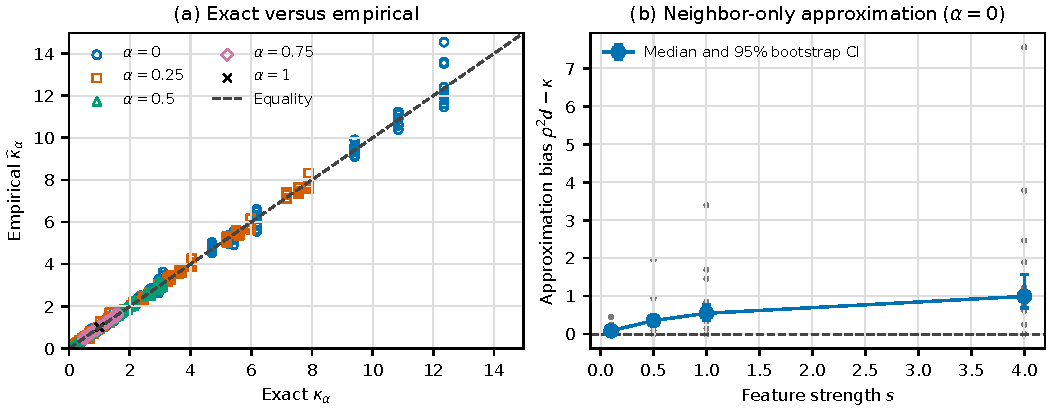
\includegraphics[width=\linewidth]{results/discriminability/route_a_grid_v1/summary/validation_figure}
\caption{Frozen moment validation. Left: empirical and exact $\kappa_\alpha$. Right: signed error of the neighbor-only $\rho^2d$ approximation, with descriptive bootstrap intervals of the median.}
\label{fig:direct_discriminability_validation}
\end{figure}

This experiment validates the implemented first- and second-moment calculation within the prescribed surrogate grid. It does not validate a Bayes-error formula, a trained-GNN performance law, or a graph-vs-MLP selector.

\subsection{Broadcasting Context, Not a GNN Threshold}

The product ``branching factor $\times$ squared label correlation'' also appears in classical tree broadcasting and reconstruction. For a regular tree with forward branching factor $b$, the Kesten--Stigum quantity is $b\rho^2$~\cite{kesten1966additional,mossel2015reconstruction}. Here $b=q-1$ for a $q$-regular undirected tree, whereas a Poisson Galton--Watson limit with mean offspring $k$ uses $b=k$. This resemblance supplies historical context for the weak-feature limit of our one-hop ratio; it is not a new threshold result. In particular, $d$ in Proposition~\ref{prop:fixed_degree} is a fixed one-hop neighbor count and must not be interchanged with either forward degree without an explicit coupling. Ordinary finite-depth GNNs also reuse neighborhoods and may include self-loops, normalization, nonlinearities, attention, and learned transformations. We therefore derive no Kesten--Stigum condition for GNN depth or architecture. Recent finite-depth CSBM analysis likewise finds Gaussian-mixture embeddings and depth behavior more complex than a single-Gaussian account~\cite{pmlr-v269-dalle25a}.

\subsection{Extensions Not Claimed Here}

A multi-class graph is described by a class-transition matrix rather than one scalar edge correlation. Collapsing that matrix to homophily can hide which class pairs are mixed and how their feature means are arranged. We therefore do not present a scalar multi-class threshold. Likewise, a practical GCN introduces variable degree, self-loop normalization, learned transformations, nonlinearities, and neighborhood reuse across layers. Proposition~\ref{prop:self_neighbor_mixing} isolates a prescribed self-feature weight but does not remove these remaining differences.

\subsection{Scope and Random-Degree Extension}

The class-conditional distribution of $A_v$ is generally a Gaussian mixture because the neighbor labels are random. Therefore the Gaussian Bayes-error formula stated for $X_v$ must not be applied to $A_v$ solely from its first two moments. Proposition~\ref{prop:fixed_degree} concerns Mahalanobis discriminability only.

For sparse CSBM, the degree is random. Conditional on $D_v=m>0$, Proposition~\ref{prop:fixed_degree} applies with $d=m$. An unconditional calculation must specify the treatment of isolated nodes and average over the degree-conditioned mixture; replacing $D_v$ by its mean is not exact. We leave that random-degree extension separate rather than attach unsupported finite-$n$ error rates to the fixed-degree result.

\section{Discussion}
\label{sec:discussion}

\subsection{What the Negative Result Establishes}

The prospective benchmark evaluates diagnostics as actions rather than as post-hoc correlates. Under the frozen 11-dataset protocol, the combined rule and the four structure-based variants do not provide stable incremental value over an always-graph policy. This conclusion is bounded to the evaluated statistics, thresholds, model portfolio, accuracy target, and one-percentage-point margin. It does not imply that every possible graph diagnostic must fail or that cross-dataset learned selectors are impossible.

The comparison also shows why trivial policies belong in diagnostic studies. Graph is the target in 89 of 110 units, making always-graph a strong reference before any structural statistic is consulted. A diagnostic that predicts the majority action on many units can appear accurate while still adding no decision value. Oracle-family regret exposes the cost of the remaining errors, and coverage prevents abstention from receiving favorable treatment. These quantities should accompany correlation whenever a graph statistic is proposed for operational selection.

\subsection{Graph Utility Is Not a Scalar Property}

The degree-preserving intervention changes the interpretation of the negative result. Large paired losses after randomization show that useful edge organization is present in Cora, CiteSeer, and PubMed even though homophily, degree, and the two-hop statistic do not yield a reliable general selector. The apparent tension is resolved if graph utility depends on interactions that low-dimensional summaries discard: class-specific mixing, feature alignment, motifs, long-range paths, architecture, and optimization can affect performance jointly. The fixed-degree analysis in Section~\ref{sec:snr} illustrates one such interaction in a controlled surrogate, but it is not a model-selection theorem.

Validation selection has the lowest descriptive regret in the benchmark, although its advantage over the combined rule does not remain significant after the predeclared Holm correction. Unlike a cheap structural rule, validation selection requires training both model families. It therefore serves as a performance reference rather than a cost-free diagnostic. A useful future selector must be evaluated against both extremes: the trivial family policy that is strong under the observed target distribution and the validation policy that spends the full training budget.

\subsection{Limitations and External Validity}

The study covers 11 public node-classification datasets, ten seeds, one stratified split design, seven architectures, four trials per architecture, and test accuracy as the outcome. The thresholds are intentionally simple and frozen; they are not optimized for each dataset. These choices make the negative result auditable but limit generalization to inductive deployment, graph-level tasks, dynamic or heterogeneous graphs, different model portfolios, and cost-sensitive objectives. The eligibility amendment also excludes Texas because its singleton class cannot support the fixed three-way split, so the benchmark does not characterize that small-data regime.

The intervention adds a different limitation. It evaluates GCN on three citation networks, leaving only three independent dataset clusters for inference. Degree preservation does not preserve connected components, homophily, motifs, spectral structure, or path statistics. The intervention therefore establishes sensitivity to non-degree edge organization, not a causal effect of any one structural attribute.

\subsection{Implications for Future Work}

The next step is not another hand-tuned threshold over the same summaries. More promising directions include learned representations of structural utility, uncertainty-aware abstention, explicit training-cost objectives, and selectors evaluated with leave-dataset-out or external prospective data. Such work should retain the safeguards used here: decision-time provenance, matched model portfolios, test-once accounting, trivial policies, regret and coverage, dataset-level inference, and immutable per-unit records.

\section{Conclusion}
\label{sec:conclusion}

This paper asks whether transparent graph diagnostics can decide when node classification should use a tuned graph-model family rather than a tuned feature-only MLP. In a frozen prospective benchmark spanning 11 datasets, ten seeds, 770 model records, and 110 diagnostic records, the historical combined rule reaches 55.5\% selection accuracy and 7.46 percentage points of full-set regret. Always-graph reaches 80.9\% and 0.26 points, while validation selection reaches 91.8\% and 0.22 points. No predeclared comparison establishes an advantage for the combined rule after Holm correction. Under this protocol, the evaluated simple diagnostics therefore provide no stable incremental decision value.

The negative decision result is not evidence that graph structure is irrelevant. Degree-preserving randomization lowers GCN accuracy by 45.5, 29.9, and 17.3 points on Cora, CiteSeer, and PubMed, respectively. Because the intervention changes several forms of edge organization and covers only three dataset clusters, it does not isolate homophily or support a universal causal claim. It instead supplies the paper's main bounded insight: graph structure can carry substantial predictive value even when low-dimensional diagnostics fail to characterize that value reliably.

Future work should evaluate richer or learned representations of graph utility under the same prospective safeguards, including matched trivial baselines, explicit abstention, regret, dataset-level inference, and immutable provenance. The scoped fixed-degree analysis offers mechanistic context for such work, but the empirical evidence argues against treating a single structural statistic as a general graph-vs-MLP selection rule.

\appendix
\setcounter{table}{0}
\section{Dataset-Level Results and Reproducibility Details}
\label{app:reproducibility}

This appendix reports descriptive heterogeneity and implementation details requested for textual reproducibility. All outcome summaries are deterministic transformations of the frozen audit; no model was retrained, no action was changed, and the primary dataset-level inference remains that in Section~\ref{sec:prospective}.

\subsection{Dataset Properties and Decision Heterogeneity}

Table~\ref{tab:dataset_properties} reports graph properties after the common canonicalization step. Here, $|E|$ counts unique undirected non-loop edges, $h_1$ is the training-label edge-homophily statistic averaged over the ten splits, and $\Delta h=h_2-h_1$ uses the path-weighted two-hop statistic defined in Section~\ref{sec:protocol}.

\begin{table}[ht]
\centering
\caption{Dataset properties and mean train-label graph diagnostics.}
\label{tab:dataset_properties}
\scriptsize
\setlength{\tabcolsep}{3.2pt}
\begin{tabular}{@{}lrrrrrrr@{}}
\toprule
Dataset & $|V|$ & $|E|$ & Classes & Features & Mean degree & $h_1$ & $\Delta h$ \\
\midrule
Actor & 7,600 & 26,659 & 5 & 932 & 7.02 & 0.219 & $-0.009$ \\
Amazon-ratings & 24,492 & 93,050 & 5 & 300 & 7.60 & 0.380 & 0.038 \\
Chameleon & 2,277 & 31,371 & 5 & 2,325 & 27.55 & 0.236 & 0.060 \\
CiteSeer & 3,327 & 4,552 & 6 & 3,703 & 2.74 & 0.732 & 0.039 \\
Coauthor-CS & 18,333 & 81,894 & 15 & 6,805 & 8.93 & 0.810 & $-0.125$ \\
Cora & 2,708 & 5,278 & 7 & 1,433 & 3.90 & 0.808 & $-0.069$ \\
Cornell & 183 & 277 & 5 & 1,703 & 3.03 & 0.114 & 0.304 \\
PubMed & 19,717 & 44,324 & 3 & 500 & 4.50 & 0.804 & $-0.024$ \\
Roman-empire & 22,662 & 32,927 & 18 & 300 & 2.91 & 0.047 & 0.024 \\
Squirrel & 5,201 & 198,353 & 5 & 2,089 & 76.27 & 0.221 & 0.014 \\
Wisconsin & 251 & 450 & 5 & 1,703 & 3.59 & 0.172 & 0.257 \\
\bottomrule
\end{tabular}
\end{table}

Table~\ref{tab:dataset_decisions} shows that the negative result is heterogeneous but not driven by a single dataset. The largest Combined losses occur on Amazon-ratings, Chameleon, Roman-empire, and Squirrel. Three of those datasets contribute 30 of the 35 abstentions, whereas Chameleon receives ten explicit MLP actions. The column ``Combined G/M/A'' gives action counts before fallback; all regrets use the frozen MLP fallback and are averaged over ten seeds.

\begin{table}[ht]
\centering
\caption{Dataset-level targets, decisions, and mean oracle-portfolio regret. G/M/A denotes graph/MLP/abstain counts before fallback; gaps and regrets are percentage points.}
\label{tab:dataset_decisions}
\scriptsize
\setlength{\tabcolsep}{3.0pt}
\begin{tabular}{@{}lrrrrrr@{}}
\toprule
Dataset & Graph targets & Mean gap & Combined G/M/A & Combined & Always-G & Validation \\
\midrule
Actor & 0/10 & 0.10 & 0/5/5 & 0.34 & 0.24 & 0.34 \\
Amazon-ratings & 10/10 & 16.45 & 0/0/10 & 16.45 & 0.00 & 0.00 \\
Chameleon & 10/10 & 15.88 & 0/10/0 & 15.88 & 0.00 & 0.00 \\
CiteSeer & 10/10 & 5.16 & 10/0/0 & 0.00 & 0.00 & 0.00 \\
Coauthor-CS & 10/10 & 4.75 & 10/0/0 & 0.00 & 0.00 & 0.00 \\
Cora & 10/10 & 12.59 & 10/0/0 & 0.00 & 0.00 & 0.00 \\
Cornell & 4/10 & 0.50 & 0/10/0 & 1.75 & 1.25 & 1.50 \\
PubMed & 10/10 & 2.01 & 10/0/0 & 0.00 & 0.00 & 0.00 \\
Roman-empire & 10/10 & 23.66 & 0/0/10 & 23.66 & 0.00 & 0.00 \\
Squirrel & 10/10 & 22.06 & 0/0/10 & 22.06 & 0.00 & 0.00 \\
Wisconsin & 5/10 & 0.57 & 0/10/0 & 1.89 & 1.32 & 0.57 \\
\bottomrule
\end{tabular}
\end{table}

\subsection{Architecture and Preprocessing Specification}

All runs use PyTorch 2.9.1 and PyTorch Geometric 2.7.0. Planetoid loads Cora, CiteSeer, and PubMed; WebKB loads Wisconsin and Cornell. WikipediaNetwork with geometric preprocessing loads Chameleon and Squirrel. Actor uses the Actor loader. Roman-empire and Amazon-ratings use PyG's Heterophilous Graph Dataset loader; Coauthor-CS uses Coauthor. The PyG \texttt{NormalizeFeatures} transform is applied on load. We then remove self-loops, collapse duplicate and reverse edges to a unique undirected edge set, and emit both directions for message passing; isolated nodes are retained. These canonical edges are also the input to the diagnostics.

Table~\ref{tab:architecture_details} completes the common training grid in Table~\ref{tab:frozen_training}. Unless stated otherwise, hidden width is 64, outputs are unnormalized logits, and dropout is the selected trial value. No architecture other than the PyG LINKX implementation uses BatchNorm.

\begin{table}[ht]
\centering
\caption{Exact architecture and propagation details used in the frozen benchmark.}
\label{tab:architecture_details}
\small
\begin{tabular}{@{}lp{0.76\linewidth}@{}}
\toprule
Model & Frozen implementation \\
\midrule
MLP & Author implementation with two affine layers, ReLU after the hidden layer, and hidden dropout; graph edges are ignored. \\
GCN & Two \texttt{GCNConv} layers, ReLU, then hidden dropout. PyG's default symmetric normalization and added self-loops are used. \\
GAT & Two \texttt{GATConv} layers: four concatenated attention heads in the first layer, ELU, hidden dropout, and one non-concatenated output head. The selected dropout is also applied to attention coefficients; PyG adds self-loops. \\
GraphSAGE & Two mean-aggregating \texttt{SAGEConv} layers with root transforms, ReLU, and hidden dropout. No explicit self-loop edges or output normalization are added. \\
H2GCN & Author implementation with a linear ReLU embedding and two propagation rounds over separately symmetrically normalized one-hop and strict two-hop adjacencies. All layer representations are concatenated, followed by dropout and a linear classifier; these fixed adjacencies contain no self-loops. \\
LINKX & PyG \texttt{LINKX} with one sparse edge layer, two node-MLP layers, and two outer layers. The PyG MLP blocks use ReLU and BatchNorm on hidden transitions; selected dropout is applied in the final MLP. \\
GPR-GNN & Author implementation with input dropout, linear--ReLU--dropout--linear prediction, and ten trainable PPR-initialized propagation coefficients ($\alpha=0.1$). Propagation uses GCN normalization with self-loops. \\
\bottomrule
\end{tabular}
\end{table}

The implementation uses full-batch training for every architecture. Cross-entropy is computed only on training indices; validation accuracy and loss select the stored checkpoint and trial as described in Section~\ref{sec:protocol}. There is no batch normalization outside LINKX, no feature augmentation beyond \texttt{NormalizeFeatures}, and no dataset-specific hyperparameter or preprocessing exception in the final v2 run.


\section*{Data and code availability}
\begin{sloppypar}
The current experiment code, frozen configurations, compact deterministic audits, and figure-generation scripts are available at \url{https://github.com/MengdanXue/prospective-graph-diagnostics}. A path-redacted archive of the immutable unit-level records is preserved in the versioned v0.1.0 release at \url{https://github.com/MengdanXue/prospective-graph-diagnostics/releases/tag/v0.1.0}. Historical exploratory outputs are separated from the confirmatory artifacts. The public repository is a fresh publication snapshot with file digests and execution-provenance mappings; it does not expose the complete history of the private predecessor repository.
\end{sloppypar}

\section*{Declaration of generative AI and AI-assisted technologies in the writing process}
During the preparation of this work, the author used OpenAI Codex to assist with software review, test development, reproducibility checks, and language and structural editing. The author independently verified all code, experimental artifacts, statistical results, references, and manuscript content and takes full responsibility for the work.

\bibliographystyle{elsarticle-num}
\bibliography{references}

\end{document}
